\documentclass{article}
\usepackage{PreambleCommon}
\usepackage{minted}


\title{Assignment 5: Big-O Sorting \\[5pt] Part 2: Miles \\[8pt] CS3305/W01 Data Structures}
\author{Casey Hampson}

\begin{document}
\maketitle


\section*{Program Output}

\begin{center}
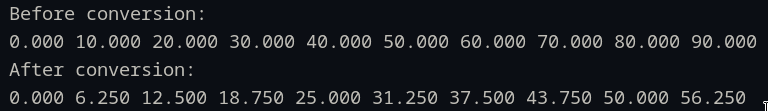
\includegraphics[width=0.9\linewidth]{res/1.png}
\end{center}

\section*{Worst Case Efficiency}
Obviously, this code is going to be $\mathcal{O}(n)$, since the conversion from miles to kilometers doesn't have any relation to the number of input parameters we have, it's just a constant time calculation. The worst-case condition would perhaps be for the largest floats possible, but even then, as just mentioned, this has no relation to the size of the input, meaning it will still be considered to run at constant time, and the entire program will still run at $\mathcal{O}(n)$. 


\pagebreak
\section*{Source Code}
\inputminted{java}{./P2.java}




\end{document}
